\chapter{Gamificação}
\label{chap:cap1}
 
Este capítulo discutirá o que é gamificação e como ela pode ser utilizada no aprendizado. Também discutirá como a gamificação pode ser aplicada em um ambiente empresarial.


\section{Gamificação do aprendizado}
\label{sec:superv}

Este capítulo apresentará como a gamificação pode ser aplicada ao aprendizado e efeito que ela tem no engajamento.


\section{Aplicações empresariais}
\label{sec:nsuperv}

Este capítulo apresentará como a gamificação pode ser utilizada em um ambiente empresarial e dando embasamento teórico de como o projeto poderia ajudar uma empresa.


% \begin{figure}[htb]
% \caption{\label{fig:comparacaoaprendizado} Comparaçao entre aprendizados}
% \begin{center}
% 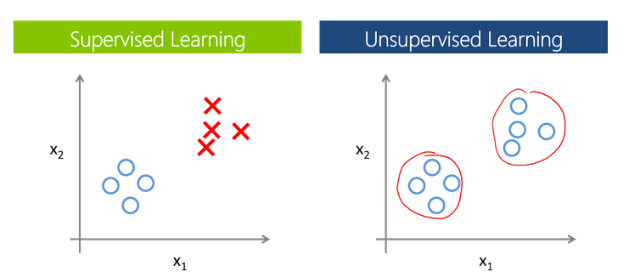
\includegraphics[scale=0.75]{ComparaAprendizado}
% \end{center}
% \legend{Fonte: \citeauthor{mediummachine}, \citeyear{mediummachine}} 
% \end{figure}

%\autoref{chap:cap1}
% ---
%\section{Aliquam vestibulum fringilla lorem}
%\lipsum[2]
%\subsection{Subsessão cap 1}
%\lipsum[2]
%\chapter{Capitulo Segundo}
%\lipsum[2]
